\documentclass[11pt, twoside, fleqn]{report}

\usepackage[backend=biber, style=ieee]{biblatex}
\usepackage[parfill, skip=1em]{parskip}
\usepackage[labelfont=bf]{caption}
\usepackage[margin=1in]{geometry}
\usepackage[hidelinks]{hyperref}
\usepackage{amssymb, booktabs, derivative, fancyhdr, float, graphicx, natex, pagecolor, pgfplots, siunitx, tikz}

% background and foreground colors
\definecolor{bgcolor}{HTML}{1e1e2e}
\definecolor{fgcolor}{HTML}{cdd6f4}

% catppuccin palette
\definecolor{p1}{HTML}{cba6f7}
\definecolor{p2}{HTML}{f38ba8}
\definecolor{p3}{HTML}{fab387}
\definecolor{p4}{HTML}{a6e3a1}
\definecolor{p5}{HTML}{89dceb}
\definecolor{p6}{HTML}{89b4fa}

% pagecolor
\pagecolor{bgcolor}
\color{fgcolor}

% biblatex
\addbibresource{references.bib}

% fancyhdr
\renewcommand{\chaptermark}[1]{\markboth{\thechapter\ #1}{}}
\renewcommand{\sectionmark}[1]{\markright{\thesection\ #1}}
\renewcommand{\footrulewidth}{0.4pt}

\fancypagestyle{mystyle}{
    \fancyfoot{}
    \fancyfoot[C]{\thepage}
}

% hyperref
\urlstyle{same}

% pgfplots
\pgfplotsset{compat=newest}

% custom
\newcommand{\dash}{\!-\!}
\newcommand{\state}[2]{\prescript{#1}{}{#2}}

\begin{document}

\pagestyle{empty}

\begin{titlepage}
    \null
    \vspace{\fill}
    \begin{center}
        \let \footnote \thanks
        {\LARGE \textbf{Simulation of Molecular Spectra} \par}
        {\large Theory and Applications}
        \vskip 1.5em
            {\large
                \lineskip .5em
                \begin{tabular}[t]{c}
                    Nathan Phillips
                \end{tabular}\par}
        \vskip 1em
            {\large \today}
        \vskip 2em
    \end{center}
    \vspace{\fill}

    \begin{center}
        {\large{\textbf{Texas A\&M University}} \par}
        {\large{Department of Aerospace Engineering}}
    \end{center}
\end{titlepage}

\tableofcontents
\newpage
\listoffigures
\newpage
\listoftables
\newpage

\pagestyle{mystyle}

\input{chapters/approximations}

\input{chapters/structure}

\input{chapters/intensities}

\input{chapters/numbers}

\input{chapters/hund}

\input{chapters/uncoupling}

\input{chapters/transitions}

\input{chapters/lif}

\input{chapters/lineshapes}

\chapter{Placeholder}

\begin{align*}
    P_{11}(J) & = \nu_{0}^{(1)} + F_{1}'(J - 1) - F_{1}''(J) \\
    Q_{11}(J) & = \nu_{0}^{(1)} + F_{1}'(J) - F_{1}''(J)     \\
    R_{11}(J) & = \nu_{0}^{(1)} + F_{1}'(J + 1) - F_{1}''(J)
\end{align*}

\begin{align*}
    P_{12}(J) & = \nu_{0}^{(1)} + F_{1}'(J - 1) - F_{2}''(J) \\
    Q_{12}(J) & = \nu_{0}^{(1)} + F_{1}'(J) - F_{2}''(J)     \\
    R_{12}(J) & = \nu_{0}^{(1)} + F_{1}'(J + 1) - F_{2}''(J)
\end{align*}

\begin{align*}
    P_{22}(J) & = \nu_{0}^{(2)} + F_{2}'(J - 1) - F_{2}''(J) \\
    Q_{22}(J) & = \nu_{0}^{(2)} + F_{2}'(J) - F_{2}''(J)     \\
    R_{22}(J) & = \nu_{0}^{(2)} + F_{2}'(J + 1) - F_{2}''(J)
\end{align*}

\begin{align*}
    P_{21}(J) & = \nu_{0}^{(2)} + F_{2}'(J - 1) - F_{1}''(J) \\
    Q_{21}(J) & = \nu_{0}^{(2)} + F_{2}'(J) - F_{1}''(J)     \\
    R_{21}(J) & = \nu_{0}^{(2)} + F_{2}'(J + 1) - F_{1}''(J)
\end{align*}

\chapter{Multiplet Term Formulas}

Following info is from \textit{Rotational Structure in the Spectra of Diatomic Molecules} by Kov\'acs.

\section{General Multiplet Term Formulas}

In the following formulae, $B = \bar{B}/hc$, $D = \bar{D}/hc$ (p. 54).

These formulae are valid for any value of $\Lambda$ and $\Sigma$. However, they rarely give values that are compatible with experimental data (p. 57) since they are general in $S$. More useful formulae can be defined that are valid for any $Y$ and $\Lambda$, but fixed in $S$ (meaning different formulae for singlet, doublet, triplet, etc. splittings).

\subsection{Hund's Case (a)}

Equation 2.1.1.9
\begin{align*}
    F_{a}(\Lambda, S, Y \gg J(J + 1)) & = \nu_{0} + A\Lambda\Sigma + B[J(J + 1) - \Omega^{2} + S(S + 1) -\Sigma^{2}] \\
                                      & + H_{a}^{c}(\Lambda, S) + H_{a}^{ss}(\Lambda, S) + H_{a}^{sr}(\Lambda, S)
\end{align*}

\subsection{Hund's Case (b)}

Equation 2.1.1.10
\begin{align*}
    F_{b}(\Lambda, S, Y \ll N(N + 1)) & = \nu_{0} + B[N(N + 1) - \Lambda^{2}] + A\Lambda^{2}\frac{J(J + 1) - N(N + 1) - S(S + 1)}{2N(N + 1)} \\
                                      & + H_{b}^{c}(\Lambda) + H_{b}^{ss}(\Lambda, S) + H_{b}^{sr}(\Lambda, S)
\end{align*}

\section{Singlet Terms}

For singlet terms, Hund's cases (a) and (b) are the same, and can therefore be obtained from Eq. 2.2.1.9 (by setting $S = \Sigma = 0$, or from 2.1.1.10 (by setting $S = 0$ and $J = N$).

Equation 2.1.2.1
\begin{equation*}
    F(J) = \nu_{0} + B[J(J + 1) - \Lambda^{2}] - D[J(J + 1) - \Lambda^{2}]^{2}
\end{equation*}

\section{Triplet Terms}

For $\state{2}{\Sigma}$ terms, $\Lambda = 0$ and $Y = 0$ (p. 63).

Equation 2.1.3.15
\begin{align*}
    F_{J - \tfrac{1}{2}}(N) = F_{1}(N) & = \nu_{0} + B_\Sigma N(N + 1) - D_\Sigma N^{2}(N + 1)^{2} + \tfrac{1}{2}\gamma N      \\
    F_{J + \tfrac{1}{2}}(N) = F_{2}(N) & = \nu_{0} + B_\Sigma N(N + 1) - D_\Sigma N^{2}(N + 1)^{2} - \tfrac{1}{2}\gamma(N + 1)
\end{align*}

\chapter{Intensity Distribution in Rotational Bands}

Following info is from \textit{Rotational Structure in the Spectra of Diatomic Molecules} by Kov\'acs.

\section{Triplet Transitions}

The following equations used in the intensity factors for triplets. For a $\state{3}{\Sigma}\dash\state{3}{\Sigma}$ transition, $\Lambda = 0$. For Hund's case (b), $Y$ can be replaced with $0$ (p. 70).

Equation 2.1.4.9
\begin{align*}
    u_{1}^\pm(J) & = \sqrt{\Lambda^{2}Y(Y - 4) + 4J^{2}} \pm \Lambda(Y - 2)       \\
    u_{3}^\pm(J) & = \sqrt{\Lambda^{2}Y(Y - 4) + 4(J + 1)^{2}} \pm \Lambda(Y - 2)
\end{align*}

Equation 2.1.4.10
\begin{align*}
    C_{1}(J) & = \Lambda^{2}Y(Y - 4)(J - \Lambda + 1)(J + \Lambda) + 2(2J + 1)(J - \Lambda)J(J + \Lambda)               \\
    C_{2}(J) & = \Lambda^{2}Y(Y - 4) + 4J(J + 1)                                                                        \\
    C_{3}(J) & = \Lambda^{2}Y(Y - 4)(J - \Lambda)(J + \Lambda + 1) + 2(2J + 1)(J - \Lambda + 1)(J + 1)(J + \Lambda + 1)
\end{align*}

For a Hund's case (b) $\state{3}{\Sigma}\dash\state{3}{\Sigma}$ transition, these become
\begin{align*}
    u_{1}^\pm(J) & = 2J       \\
    u_{3}^\pm(J) & = 2(J + 1)
\end{align*}

And
\begin{align*}
    C_{1}(J) & = 2J^{3}(2J + 1)       \\
    C_{2}(J) & = 4J(J + 1)            \\
    C_{3}(J) & = 2(J + 1)^{3}(2J + 1)
\end{align*}

Table 3.8
\begin{table}[H]
    \centering
    \caption{Line strengths of triplet transitions for a Hund's case (b) $\state{3}{\Sigma}\dash\state{3}{\Sigma}$ transition.}
    \begin{tabular}{cc}
        \toprule
        Branches   & Line Strength                                                                                                                                                      \\
        \midrule
        $P_{1}(J)$ & $\dfrac{J[(J^{2} - 1)u'^{+}_{1}(J - 1)u''^{+}_{1}(J) + (J^{2} - 1)u'^{-}_{1}(J - 1)u''^{-}_{1}(J) + 8J^{2}(J - 1)^{2}]^{2}}{16C'_{1}(J - 1)C''_{1}(J)}$            \\
        \addlinespace[0.5em]
        $Q_{1}(J)$ & $\dfrac{(2J + 1)[-J(J + 1)u'^{+}_{1}(J)u''^{+}_{1}(J) + J(J + 1)u'^{-}_{1}(J)u''^{-}_{1}(J)]^{2}}{16J(J + 1)C'_{1}(J)C''_{1}(J)}$                                  \\
        \addlinespace[0.5em]
        $R_{1}(J)$ & $\dfrac{(J + 1)^{2}[J(J + 2)u'^{+}_{1}(J + 1)u''^{+}_{1}(J) + J(J + 2)u'^{-}_{1}(J + 1)u''^{-}_{1}(J) + 8J^{2}(J + 1)^{2}]^{2}}{16(J + 1)C'_{1}(J + 1)C''_{1}(J)}$ \\
        \bottomrule
    \end{tabular}
\end{table}

\chapter{Temporary}

\section{Term Values}

Dunham series expansion from Herzberg, p. 108:
\begin{equation*}
    T = \sum_{\ell j}Y_{\ell j}\ab(v + \tfrac{1}{2})^\ell [J(J + 1)]^{j}
\end{equation*}

Coefficients From Babou, 2009:
\begin{table}[H]
    \centering
    \caption{Dunham Expansion Coefficients}
    \begin{tabular}{c|ccccc}
        \toprule
        $\ell$ & $j = 0$           & $j = 1$           & $j = 2$      & $j = 3$ & $j = 4$ \\
        \midrule
        0      & $Y_{00}$          & $B_{e}$           & $-D_{e}$     & $H_{e}$ & $L_{e}$ \\
        1      & $-\omega_{e}$     & $-\alpha_{e}$     & $-\beta_{e}$ &         &         \\
        2      & $\omega_{e}x_{e}$ & $\gamma_{e}$      & $-g_{e}$     &         &         \\
        3      & $\omega_{e}y_{e}$ & $\delta_{e}$      & $-h_{e}$     &         &         \\
        4      & $\omega_{e}z_{e}$ & $\varepsilon_{e}$ & $-k_{e}$     &         &         \\
        5      & $\omega_{e}a_{e}$ & $\xi_{e}$         &              &         &         \\
        6      & $\omega_{e}b_{e}$ & $\eta_{e}$        &              &         &         \\
        7      & $\omega_{e}c_{e}$ & $\theta_{e}$      &              &         &         \\
        8      & $\omega_{e}d_{e}$ &                   &              &         &         \\
        9      & $\omega_{e}e_{e}$ &                   &              &         &         \\
        \bottomrule
    \end{tabular}
\end{table}

Zero-point energy from Herzberg p. 108:
\begin{equation*}
    Y_{00} = \frac{B_{e}}{4} + \frac{\alpha_{e}\omega_{e}}{12B_{e}} + \frac{\alpha_{e}^{2}\omega_{e}^{2}}{144B_{e}^{2}} - \omega_{e}x_{e}
\end{equation*}

From Babou, 2009:
\begin{equation*}
    T = T_{e} + G + F
\end{equation*}
where
\begin{align*}
    G = \omega_{e}\ab(v + \tfrac{1}{2}) & - \omega_{e}x_{e}\ab(v + \tfrac{1}{2})^{2} + \omega_{e}y_{e}\ab(v + \tfrac{1}{2})^{3} + \omega_{e}z_{e}\ab(v + \tfrac{1}{2})^{4} + \omega_{e}a_{e}\ab(v + \tfrac{1}{2})^{5}          \\
                                        & + \omega_{e}b_{e}\ab(v + \tfrac{1}{2})^{6} + \omega_{e}c_{e}\ab(v + \tfrac{1}{2})^{7} + \omega_{e}d_{e}\ab(v + \tfrac{1}{2})^{8} + \omega_{e}e_{e}\ab(v + \tfrac{1}{2})^{9} + \dotsb
\end{align*}
and (generally)
\begin{equation*}
    F = B_{v}J(J + 1) + D_{v}[J(J + 1)]^{2} + H_{v}[J(J + 1)]^{3} + \dotsb
\end{equation*}

The rotational constants are
\begin{align*}
    B_{v} = B_{e} & - \alpha_{e}\ab(v + \tfrac{1}{2}) + \gamma_{e}\ab(v + \tfrac{1}{2})^{2} + \delta_{e}\ab(v + \tfrac{1}{2})^{3} + \varepsilon_{e}\ab(v + \tfrac{1}{2})^{4} + \xi_{e}\ab(v + \tfrac{1}{2})^{5} + \eta_{e}\ab(v + \tfrac{1}{2})^{6} \\
                  & + \theta_{e}\ab(v + \tfrac{1}{2})^{7} + \dotsb
\end{align*}
and
\begin{equation*}
    D_{v} = D_{e} + \beta_{e}\ab(v + \tfrac{1}{2}) + g_{e}\ab(v + \tfrac{1}{2})^{2} + h_{e}\ab(v + \tfrac{1}{2})^{3} + k_{e}\ab(v + \tfrac{1}{2})^{4} + \dotsb
\end{equation*}
and
\begin{equation*}
    H_{v} = H_{e} + \dotsb
\end{equation*}

From \textit{Molecular Spectroscopic Constants of O$_{2}$ (B$\state{3}{\Sigma}^{-}_{u}$): The Upper State of the Schumann--Runge Bands} by Cheung, Eq. (1):
\begin{equation*}
    \sop{H} = B\vb{N}^{2} + \tfrac{2}{3}\lambda(3S_{z}^{2} - \vb{S}^{2}) + \gamma\vb{N}\vdot\vb{S}
\end{equation*}
where
\begin{equation*}
    \vb{N} = \vb{J} - \vb{S}
\end{equation*}

Which can be expressed as (Wilheit, 1969 Eq. 1)
\begin{align*}
    \sop{H} = B\pmx{
    J(J - 1)                           & 0                                        & 0            \\
    (J + 1)(J + 2)                     & 0                                                       \\
    0                                  & 0                                        & J(J + 1)
    }
                                       & + \lambda\pmx{
    \tfrac{-2J}{2J + 1} + \tfrac{2}{3} & \tfrac{2\sqrt{J(J + 1)}}{2J + 1}         & 0            \\
    \tfrac{2\sqrt{J(J + 1)}}{2J + 1}   & \tfrac{-2(J + 1)}{2J + 1} + \tfrac{2}{3} & 0            \\
    0                                  & 0                                        & \tfrac{2}{3}
    }                                                                                            \\
                                       & + \gamma\pmx{
    J - 1                              & 0                                        & 0            \\
    0                                  & -(J + 2)                                 & 0            \\
    0                                  & 0                                        & 1
    }
\end{align*}
where (Krupiene Appendix C)
\begin{align*}
    B       & = B_{0} + B_{1}N(N + 1)             \\
    \lambda & = \lambda_{0} + \lambda_{1}N(N + 1) \\
    \gamma  & = \gamma_{0} + \gamma_{1}N(N + 1)
\end{align*}
Note that $B_{1} = -D_{0}$

Cheung, Table 1:
\begin{equation*}
    x = J(J + 1)
\end{equation*}
and
\begin{equation*}
    F_{2} = T + Bx - Dx^{2} + \tfrac{2}{3}\lambda - \gamma + \tfrac{2}{3}\lambda_{D}x - \gamma_{D}x
\end{equation*}
The matrix elements of the Hamiltonian are symmetric
\begin{equation*}
    \bmx{H_{11} & H_{12} \\ H_{21} & H_{22}}
\end{equation*}
where
\begin{align*}
    H_{11} & = T + B(x + 2) - D(x^{2} + 8x + 4) - \tfrac{4}{3}\lambda - 2\gamma - \tfrac{4}{3}\lambda_{D}(x + 2) - 4\gamma_{D}(x + 1) \\
    H_{12} & = -2\sqrt{x}\ab[B - 2D(x + 1) - \tfrac{\gamma}{2} - \tfrac{2}{3}\lambda_{D} - \tfrac{1}{2}\gamma_{D}(x + 4)]             \\
    H_{21} & = H_{12}                                                                                                                 \\
    H_{22} & = T + Bx - D(x^{2} + 4x) + \tfrac{2}{3}\lambda - \gamma + \tfrac{2}{3}x\lambda_{D} - 3x\gamma_{D}
\end{align*}
The eigenvalues are
\begin{align*}
    F_{1}, F_{3} = & -\tfrac{3}{2}\gamma - \tfrac{7}{2}\gamma_{D} x - 2 \gamma_{D} - \tfrac{1}{3}\lambda - \tfrac{1}{3}\lambda_{D} x - \tfrac{4}{3}\lambda_{D} + B x + B - D x^{2} - 6 D x - 2 D + T                           \\
                   & \pm \tfrac{1}{6}\bigl(36 \gamma^{2} x + 9 \gamma^{2} + 72 \gamma \gamma_{D} x^{2} + 306 \gamma \gamma_{D} x + 72 \gamma \gamma_{D} + 36 \gamma \lambda + 132 \gamma \lambda_{D} x + 48 \gamma \lambda_{D} \\
                   & - 144 \gamma B x - 36 \gamma B + 288 \gamma D x^{2} + 360 \gamma D x + 72 \gamma D + 36 \gamma_{D}^{2} x^{3} + 297 \gamma_{D}^{2} x^{2} + 648 \gamma_{D}^{2} x                                            \\
                   & + 144 \gamma_{D}^{2} + 36 \gamma_{D} \lambda x + 144 \gamma_{D} \lambda + 132 \gamma_{D} \lambda_{D} x^{2} + 576 \gamma_{D} \lambda_{D} x + 192 \gamma_{D} \lambda_{D} - 144 \gamma_{D} B x^{2}           \\
                   & - 612 \gamma_{D} B x - 144 \gamma_{D} B + 288 \gamma_{D} D x^{3} + 1512 \gamma_{D} D x^{2} + 1512 \gamma_{D} D x + 288 \gamma_{D} D + 36 \lambda^{2}                                                      \\
                   & + 72 \lambda \lambda_{D} x + 96 \lambda \lambda_{D} - 72 \lambda B + 144 \lambda D x + 144 \lambda D + 36 \lambda_{D}^{2} x^{2} + 160 \lambda_{D}^{2} x + 64 \lambda_{D}^{2}                              \\
                   & - 264 \lambda_{D} B x - 96 \lambda_{D} B + 528 \lambda_{D} D x^{2} + 720 \lambda_{D} D x + 192 \lambda_{D} D + 144 B^{2} x + 36 B^{2}                                                                     \\
                   & - 576 B D x^{2} - 720 B D x - 144 B D + 576 D^{2} x^{3} + 1296 D^{2} x^{2} + 864 D^{2} x + 144 D^{2}\bigr)^{1/2}
\end{align*}

\section{H\"onl--London Factors}

From \textit{H\"onl--London Factors for $\state{3}{\Sigma}^\pm\dash\state{3}{\Sigma}^\pm$ Transitions} by Tatum, Table 1:
\begin{table}[H]
    \centering
    \caption{H\"onl--London Factors for $\state{3}{\Sigma}^\pm\dash\state{3}{\Sigma}^\pm$ Transitions}
    \begin{tabular}{ccc}
        \toprule
        Branch              & Emission                                & Absorption                                 \\
        \midrule
        $P_{1}$             & $\dfrac{(N' + 1)(2N' + 5)}{2N' + 3}$    & $\dfrac{N''(2N'' + 3)}{2N'' + 1}$          \\
        \addlinespace[0.5em]
        $R_{1}$             & $\dfrac{N'(2N' + 3)}{2N' + 1}$          & $\dfrac{(N'' + 1)(2N'' + 5)}{2N'' + 3}$    \\
        \addlinespace[0.5em]
        $\state{P}{R}_{13}$ & $\dfrac{1}{(N' + 1)(2N' + 1)(2N' + 3)}$ & $\dfrac{1}{N''(2N'' - 1)(2N'' + 1)}$       \\
        \addlinespace[0.5em]
        $\state{P}{Q}_{12}$ & $\dfrac{1}{N' + 1}$                     & $\dfrac{1}{N''}$                           \\
        \addlinespace[0.5em]
        $P_{2}$             & $\dfrac{N'(N' + 2)}{N' + 1}$            & $\dfrac{(N'' - 1)(N'' + 1)}{N''}$          \\
        \addlinespace[0.5em]
        $R_{2}$             & $\dfrac{(N' - 1)(N' + 1)}{N'}$          & $\dfrac{N''(N'' + 2)}{N'' + 1}$            \\
        \addlinespace[0.5em]
        $\state{P}{Q}_{23}$ & $\dfrac{1}{N' + 1}$                     & $\dfrac{1}{N''}$                           \\
        \addlinespace[0.5em]
        $\state{R}{Q}_{21}$ & $\dfrac{1}{N'}$                         & $\dfrac{1}{N'' + 1}$                       \\
        \addlinespace[0.5em]
        $P_{3}$             & $\dfrac{(N' + 1)(2N' - 1)}{2N' + 1}$    & $\dfrac{N''(2N'' - 3)}{2N'' - 1}$          \\
        \addlinespace[0.5em]
        $R_{3}$             & $\dfrac{N'(2N' - 3)}{2N' - 1}$          & $\dfrac{(N'' + 1)(2N'' - 1)}{2N'' + 1}$    \\
        \addlinespace[0.5em]
        $\state{R}{Q}_{32}$ & $\dfrac{1}{N'}$                         & $\dfrac{1}{N'' + 1}$                       \\
        \addlinespace[0.5em]
        $\state{R}{P}_{31}$ & $\dfrac{1}{N'(2N' - 1)(2N' + 1)}$       & $\dfrac{1}{(N'' + 1)(2N'' + 1)(2N'' + 3)}$ \\
        \bottomrule
    \end{tabular}
\end{table}

\section{Spectral Lineshapes}

\subsection{Lorentzian Profile}

From \textit{A Student's Guide to Atomic Physics} by Fox, Eq. (3.31) and \textit{Spectroscopy and Optical Diagnostics for Gases} by Hanson, Eq. (8.7):
\begin{equation*}
    \phi_{L}(\nu) = \frac{1}{2\pi}\frac{\adif{\nu}}{(\nu - \nu_{0})^{2} + (\adif{\nu}/2)^{2}}
\end{equation*}

From \textit{A Student's Guide to Atomic Physics} by Fox, Eq. (3.32) and \textit{Spectroscopy and Optical Diagnostics for Gases} by Hanson, Eq. (8.6):
\begin{equation*}
    \adif{\nu} = \frac{1}{2\pi}\ab(\frac{1}{\tau'} + \frac{1}{\tau''})
\end{equation*}

\subsection{Natural Broadening}

From \textit{Spectroscopy and Optical Diagnostics for Gases} by Hanson, Eq. (8.11):
\begin{equation*}
    \adif{\nu}_{N} = \frac{1}{2\pi}\ab(\sum_{k} A_{ik} + \sum_{k} A_{jk})
\end{equation*}

\subsection{Collisional Broadening}

From \textit{A Student's Guide to Atomic Physics} by Fox, Eq. (3.35) and \textit{Spectroscopy and Optical Diagnostics for Gases} by Hanson, Eq. (8.17):
\begin{equation*}
    \adif{\nu}_{C} = \frac{p\sigma_{c}}{2\pi}\sqrt{\frac{8}{\pi\mu_{12}k_{B}T}}
\end{equation*}

From \textit{Spectroscopy and Optical Diagnostics for Gases} by Hanson, Eq. (8.12) and Plasma Physics Slideset 5, page 5:
\begin{equation*}
    \sigma_{c} = \pi d_{12}^{2} = \pi\ab(\frac{d_{1} + d_{2}}{2})^{2}
\end{equation*}

From \textit{Spectroscopy and Optical Diagnostics for Gases} by Hanson, Eq. (8.15):
\begin{equation*}
    \mu_{12} = \frac{m_{1}m_{2}}{m_{1} + m_{2}}
\end{equation*}

\subsection{Gaussian Profile}

From \textit{A Student's Guide to Atomic Physics} by Fox, Eq. (3.42) and \textit{Spectroscopy and Optical Diagnostics for Gases} by Hanson, Eq. (8.22):
\begin{equation*}
    \phi_{G}(\nu) = \frac{2}{\adif{\nu}}\sqrt{\frac{\ln{2}}{\pi}}\exp\ab[-4\ln{2}\ab(\frac{\nu - \nu_{0}}{\adif{\nu}})^{2}]
\end{equation*}

\subsection{Doppler Broadening}

From \textit{A Student's Guide to Atomic Physics} by Fox, Eq. (3.43) and \textit{Spectroscopy and Optical Diagnostics for Gases} by Hanson, Eq. (8.24):
\begin{equation*}
    \adif{\nu}_{D} = \nu_{0}\sqrt{\frac{8kT\ln{2}}{mc^{2}}}
\end{equation*}

\section{Transition Intensities}

\subsection{Inner Product}

From \textit{Introduction to Quantum Mechanics} by Griffiths, Eq. (3.6):
\begin{equation*}
    \ip{f}{g} = \int_{a}^{b} \cc{f}g \odif{x}
\end{equation*}

\subsection{Transition Moment}

From Herzberg, Eq. (IV, 67):
\begin{equation*}
    \vb{R} = \int \psi'\vb{M}\psi'' \odif{\tau}
\end{equation*}

From Herzberg, Eq. (VI, 58): (non-degenerate only?)
\begin{equation*}
    \vb{R} = \vb{R}_{e}^{nm}\vb{R}_{v}^{v'v''}\vb{R}_{r}^{J'J''}
\end{equation*}

\section{Partition Functions}

\subsection{General Form}

General form of the Boltzmann population distribution Hanson Eq. (1.11):
\begin{equation*}
    \frac{N_{i}}{N} = \frac{g_{i}}{Q}\exp\ab(-\frac{\varepsilon_{i}}{kT})
\end{equation*}
General form of the partition function Hanson Eq. (1.12):
\begin{equation*}
    Q = \sum_{i} g_{i}\exp\ab(-\frac{\varepsilon_{i}}{kT})
\end{equation*}
The total molecular partition function can be expressed as the product of the individual translational, electronic, vibrational, rotational, and nuclear components for symmetric molecules Hanson Eq. (5.4):
\begin{equation*}
    Q = Q_{t}Q_{e}Q_{v}Q_{r}Q_{n}
\end{equation*}

\subsection{Nuclear}

Nuclear partition function for a molecule Hanson Eq. (5.9):
\begin{equation*}
    Q_{n} = \prod_{i = 1}^{L} (2I_{n} + 1)
\end{equation*}

\subsection{Rotational}
Because of the rotational symmetry of certain molecules, a symmetry parameter $\sigma$ must be added to the rotational partition function to account for the multiple molecular orientations that are indistinguishable.
Herzberg Eq. (III, 164):
\begin{equation*}
    Q_{r} = \frac{1}{\sigma} \sum g_{r}\exp\ab(-\frac{\varepsilon_{r}}{kT})
\end{equation*}
The degeneracy of each state is
\begin{equation*}
    g_{r} = 2J + 1
\end{equation*}
and the rotational energy can be expressed as the term value
\begin{equation*}
    \varepsilon_{r} = F(J)hc.
\end{equation*}
Therefore, the rotational partition function is
\begin{equation*}
    Q_{r} = \frac{1}{\sigma} \sum (2J + 1)\exp\ab(-\frac{F(J)hc}{kT}).
\end{equation*}
For sufficiently large $T$ or small $B$,
Rotational partition function for a molecule in the high-temperature limit Hanson Eq. (2.21) and Herzberg Eq. (III, 166):
\begin{equation*}
    Q_{r} \approx \frac{1}{\sigma} \int_{0}^{\infty} (2J + 1)\exp\ab(-\frac{BJ(J + 1)hc}{kT}) \odif{J} = \frac{1}{\sigma}\frac{kT}{hcB}
\end{equation*}
The Boltzmann fraction is then
\begin{equation*}
    \frac{N_{J}}{N} = \frac{(2J + 1)}{Q_{r}}\exp\ab(-\frac{F(J)hc}{kT})
\end{equation*}

\subsection{Effective Rotational}

The effective rotational partition function for symmetric molecules is Hanson Eq. (5.5):
\begin{equation*}
    Q'_{r} = Q_{r}Q_{n}
\end{equation*}
Similarly, the effective rotational degeneracy is Hanson Eq. (5.6):
\begin{equation*}
    g'_{r} = g_{r}g_{n}
\end{equation*}

\subsection{Vibrational}

Herzberg Eq. (III, 159)
\begin{equation*}
    Q_{v} = \sum g_{v}\exp\ab(-\frac{\varepsilon_{v}}{kT})
\end{equation*}
The vibrational degeneracy of each state is
\begin{equation*}
    g_{v} = 1,
\end{equation*}
and the vibrational energy can be expressed as the term value
\begin{equation*}
    \varepsilon_{v} = G(v)hc.
\end{equation*}
Therefore, the vibrational partition function is
\begin{equation*}
    Q_{v} = \sum \exp\ab(-\frac{G(v)hc}{kT}).
\end{equation*}
The Boltzmann fraction is then
\begin{equation*}
    \frac{N_{v}}{N} = \frac{1}{Q_{v}}\exp\ab(-\frac{G(v)hc}{kT})
\end{equation*}

\subsection{Electronic}

Anderson Eq. (11.56)
\begin{equation*}
    Q_{e} = \sum g_{e}\exp\ab(-\frac{\varepsilon}{kT})
\end{equation*}
The electronic degeneracy depends on the individual states. The electronic energy can be expressed as the term value
\begin{equation*}
    \varepsilon_{e} = T_{e}hc.
\end{equation*}
Therefore, the electronic partition function is
\begin{equation*}
    Q_{e} = \sum g_{e}\exp\ab(-\frac{T_{e}hc}{kT}).
\end{equation*}

\subsection{Translation}

Anderson Eq. (11.53)
\begin{equation*}
    Q_{t} = \ab(\frac{2\pi mkT}{h^{2}})^{3/2}V,
\end{equation*}
where $V$ is the volume of the system.

\section{Rate Equations}

\begin{figure}[H]
    \centering
    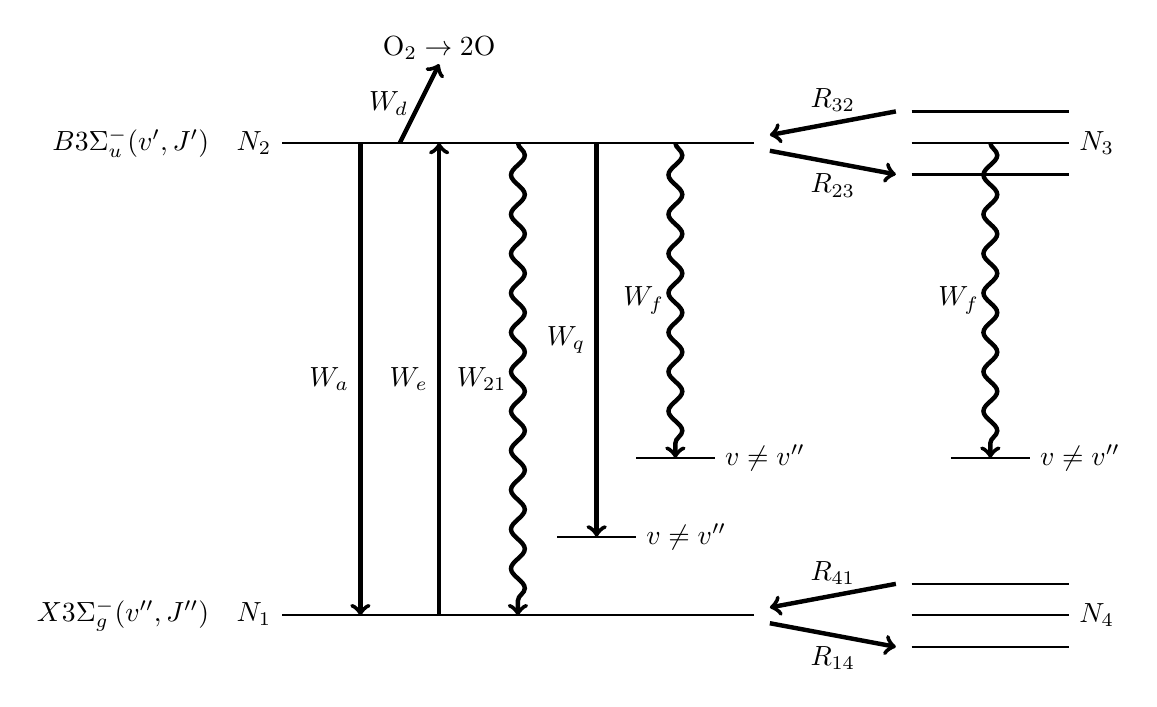
\begin{tikzpicture}
        \draw[thick] (6,0) -- (0,0) node[left] {$X\state{3}{\Sigma}_{g}^{-}(v'', J'') \quad N_{1}$};
        \draw[thick] (6,6) -- (0,6) node[left] {$B\state{3}{\Sigma}_{u}^{-}(v', J') \quad N_{2}$};

        \draw[->,ultra thick] (1,6) -- (1,0) node[midway,left] {$W_{a}$};
        \draw[->,ultra thick] (1.5,6) -- (2,7) node[midway,left] {$W_{d}$};
        \node at(2,7.2) {O$_{2} \rightarrow 2$O};
        \draw[->,ultra thick] (2,0) -- (2,6) node[midway,left] {$W_{e}$};
        \draw[->,ultra thick,decorate,decoration={snake,segment length=5mm}] (3,6) -- (3,0) node[midway,left] {$W_{21}$};
        \draw[->,ultra thick] (4,6) -- (4,1) node[midway,left] {$W_{q}$};
        \draw[thick] (3.5,1) -- (4.5,1) node[right] {$v \neq v''$};
        \draw[->,ultra thick,decorate,decoration={snake, segment length=5mm}] (5,6) -- (5,2) node[midway,left] {$W_{f}$};
        \draw[thick] (4.5,2) -- (5.5,2) node[right] {$v \neq v''$};

        \draw[<-,ultra thick] (6.2,6.1) -- (7.8,6.4) node[midway,above] {$R_{32}$};
        \draw[thick] (8,6.4) -- (10,6.4);
        \draw[thick] (8,6) -- (10,6) node[right] {$N_{3}$};
        \draw[thick] (8,5.6) -- (10,5.6);
        \draw[->,ultra thick] (6.2,5.9) -- (7.8,5.6) node[midway,below] {$R_{23}$};

        \draw[->,ultra thick,decorate,decoration={snake,segment length=5mm}] (9,6) -- (9,2) node[midway,left] {$W_{f}$};
        \draw[thick] (8.5,2) -- (9.5,2) node[right] {$v \neq v''$};

        \draw[<-,ultra thick] (6.2,0.1) -- (7.8,0.4) node[midway,above] {$R_{41}$};
        \draw[thick] (8,0.4) -- (10,0.4);
        \draw[thick] (8,0) -- (10,0) node[right] {$N_{4}$};
        \draw[thick] (8,-0.4) -- (10,-0.4);
        \draw[->,ultra thick] (6.2,-0.1) -- (7.8,-0.4) node[midway,below] {$R_{14}$};
    \end{tikzpicture}
\end{figure}

\subsection{Four-level LIF}

Gristead thesis, Eq. (2.9)
\begin{align*}
    \odv{N_{1}}{t} & = -(W_{a} + R_{14})N_{1} + (W_{e} + W_{21})N_{2} + R_{41}N_{4}                      \\
    \odv{N_{2}}{t} & = W_{a}N_{1} - (W_{f} + W_{d} + W_{q} + W_{e} + W_{21} + R_{23})N_{2} + R_{32}N_{3} \\
    \odv{N_{3}}{t} & = R_{23}N_{2} - (W_{f} + R_{32})N_{3}                                               \\
    \odv{N_{4}}{t} & = R_{14}N_{1} - R_{41}N_{4}
\end{align*}
$W_{a}$ is the laser-stimulated absorption rate, $W_{e}$ the laser-stimulated emission rate, $W_{21}$ the spontaneous emission rate, $W_{d}$ the predissociation rate, $W_{q}$ the collisional quenching rate, $W_{f}$ the fluorescent radiative decay rate, and $R_{ij}$ the rotational energy transfer rates.

\subsection{Three-level LIF}

Diskin, 1996 Eqs. (1-3)
\begin{align*}
    \odv{N_{1}}{t} & = -W_{a}N_{1} + (W_{e} + W_{21})N_{2} + W_{c}\ab(\frac{f_{b}}{1 - f_{b}}N_{3} - N_{1}) \\
    \odv{N_{2}}{t} & = W_{a}N_{1} - (W_{e} + W_{d} + W_{21} + W_{f} + W_{q})N_{2}                           \\
    \odv{N_{3}}{t} & = -W_{c}\ab(\frac{f_{b}}{1 - f_{b}}N_{3} - N_{1})
\end{align*}

\appendix
\chapter{Diatomic Constants}
\label{a:diatomic_constants}

\begin{table}[H]
    \centering
    \caption{Diatomic constants for $^{16}\mathrm{O}_{2}$ \cite{nist:diatomic}.}
    \label{t:diatomic_constants_for_o2}
    \begin{tabular}{cccc}
        \toprule
        Symbol            & \multicolumn{2}{c}{State} & Units                                        \\
        \cmidrule(lr){2-3}
                          & $X~^{3}\Sigma_{g}^{-}$    & $B~^{3}\Sigma_{u}^{-}$    &                  \\
        \midrule
        \multicolumn{4}{c}{\textit{Electronic}}                                                      \\
        \cmidrule(lr){1-4}
        $T_{e}$           & $0$                       & $49793.28$                & $\unit{cm^{-1}}$ \\
        \multicolumn{4}{c}{\textit{Vibrational}}                                                     \\
        \cmidrule(lr){1-4}
        $\omega_{e}$      & $1580.19_{3}$             & $709.31$                  & $\unit{cm^{-1}}$ \\
        $\omega_{e}x_{e}$ & $11.98_{1}$               & $10.65$                   & $\unit{cm^{-1}}$ \\
        $\omega_{e}y_{e}$ & $0.0474_{7}$              & $-0.139$                  & $\unit{cm^{-1}}$ \\
        $\omega_{e}z_{e}$ & $-0.00127_{3}$            & $-$                       & $\unit{cm^{-1}}$ \\
        \multicolumn{4}{c}{\textit{Rotational}}                                                      \\
        \cmidrule(lr){1-4}
        $B_{e}$           & $[1.4376766]$             & $0.8190_{2}$              & $\unit{cm^{-1}}$ \\
        $\alpha_{e}$      & $0.0159_{3}$              & $0.01206$                 & $\unit{cm^{-1}}$ \\
        $\gamma_{e}$      & $-$                       & $-5.5_{6}\times\num{e-4}$ & $\unit{cm^{-1}}$ \\
        $\delta_{e}$      & $-$                       & $-$                       & $\unit{cm^{-1}}$ \\
        \multicolumn{4}{c}{\textit{Centrifugal Distortion}}                                          \\
        \cmidrule(lr){1-4}
        $D_{e}$           &                           &                           & $\unit{cm^{-1}}$ \\
        $\beta_{e}$       &                           &                           & $\unit{cm^{-1}}$ \\
        \multicolumn{4}{c}{\textit{Spin-Splitting}}                                                  \\
        \cmidrule(lr){1-4}
        $\lambda$         &                           &                           & $\unit{cm^{-1}}$ \\
        $\gamma$          &                           &                           & $\unit{cm^{-1}}$ \\
        \multicolumn{4}{c}{\textit{Other}}                                                           \\
        \cmidrule(lr){1-4}
        $H_{e}$           &                           &                           & $\unit{cm^{-1}}$ \\
        $r_{e}$           &                           &                           & \AA              \\
        $\nu_{00}$        &                           &                           & $\unit{cm^{-1}}$ \\
        \bottomrule
    \end{tabular}
\end{table}

\chapter{Notation for Diatomic Constants}
\label{a:notation_for_diatomic_constants}

\begin{table}[H]
    \centering
    \caption{Notation for diatomic constants \cite{herzberg:diatomic,nist:sigma1,nist:sigma3}.}
    \label{t:notation}
    \begin{tabular}{clc}
        \toprule
        Symbol            & Definition                                                                  & Units            \\
        \midrule
        \multicolumn{3}{c}{\textit{Electronic}}                                                                            \\
        \cmidrule(lr){1-3}
        $T_{e}$           & Minimum electronic energy                                                   & $\unit{cm^{-1}}$ \\
        \multicolumn{3}{c}{\textit{Vibrational}}                                                                           \\
        \cmidrule(lr){1-3}
        $G$               & Vibrational energy                                                          & $\unit{cm^{-1}}$ \\
        $\omega_{e}$      & Vibrational constant - first term                                           & $\unit{cm^{-1}}$ \\
        $\omega_{e}x_{e}$ & Vibrational constant - second term                                          & $\unit{cm^{-1}}$ \\
        $\omega_{e}y_{e}$ & Vibrational constant - third term                                           & $\unit{cm^{-1}}$ \\
        $\omega_{e}z_{e}$ & Vibrational constant - fourth term                                          & $\unit{cm^{-1}}$ \\
        \multicolumn{3}{c}{\textit{Rotational}}                                                                            \\
        \cmidrule(lr){1-3}
        $B_{e}$           & Rotational constant - equilibrium                                           & $\unit{cm^{-1}}$ \\
        $\alpha_{e}$      & Rotational constant - first term                                            & $\unit{cm^{-1}}$ \\
        $\gamma_{e}$      & Rotational constant - second term (rotation-vibration interaction constant) & $\unit{cm^{-1}}$ \\
        $\delta_{e}$      & Rotational constant - third term                                            & $\unit{cm^{-1}}$ \\
        \multicolumn{3}{c}{\textit{Centrifugal Distortion}}                                                                \\
        \cmidrule(lr){1-3}
        $D_{e}$           & Centrifugal distortion constant - equilibrium                               & $\unit{cm^{-1}}$ \\
        $\beta_{e}$       & Centrifugal distortion constant - first term                                & $\unit{cm^{-1}}$ \\
        \multicolumn{3}{c}{\textit{Spin-Splitting}}                                                                        \\
        \cmidrule(lr){1-3}
        $\lambda$         & Spin-spin coupling parameter                                                & $\unit{cm^{-1}}$ \\
        $\gamma$          & Spin-rotation coupling parameter                                            & $\unit{cm^{-1}}$ \\
        \multicolumn{3}{c}{\textit{Other}}                                                                                 \\
        \cmidrule(lr){1-3}
        $H_{e}$           & Sixth-order rotational constant                                             & $\unit{cm^{-1}}$ \\
        $r_{e}$           & Equilibrium internuclear distance                                           & \AA              \\
        $\nu_{00}$        & Position of $0\dash0$ band                                                  & $\unit{cm^{-1}}$ \\
        \bottomrule
    \end{tabular}
\end{table}

\chapter{Quantum Numbers}
\label{a:quantum_numbers}

\begin{table}[H]
    \centering
    \caption{Various quantum numbers.}
    \label{t:quantum_numbers}
    \begin{tabular}{clc}
        \toprule
        Symbol    & Definition                            & Values                                      \\
        \midrule
        \multicolumn{3}{c}{\textit{Single Electron in Atoms}}                                           \\
        \cmidrule(lr){1-3}
        $n$       & Principal                             & $1, 2, \dotsb$                              \\
        $l$       & Azimuthal                             & $0, 1, \dotsb, (n - 1)$                     \\
        $m_{l}$   & Magnetic                              & $-l, \dotsb, l$                             \\
        $m_{s}$   & Spin                                  & $\pm \frac{1}{2}$                           \\
        \multicolumn{3}{c}{\textit{Single Electron in Molecules}}                                       \\
        \cmidrule(lr){1-3}
        $\lambda$ & Orbital Angular Momentum              & $\abs{m_{l}}$                               \\
        \multicolumn{3}{c}{\textit{Whole Atoms}}                                                        \\
        \cmidrule(lr){1-3}
        $S$       & Resultant Spin                        & $\sum s_{i}$                                \\
        $L$       & Resultant Orbital Angular Momentum    & $\sum l_{i}$                                \\
        $J$       & Total Angular Momentum                & $(L + S), (L + S - 1), \dotsb, \abs{L - S}$ \\
        $I$       & Nuclear Spin                          & ?                                           \\
        $F$       & Total Angular Momentum w/ Spin        & $(J + I), (J + I - 1), \dotsb, \abs{J - I}$ \\
        \multicolumn{3}{c}{\textit{Whole Molecules}}                                                    \\
        \cmidrule(lr){1-3}
        $M_{L}$   & ?                                     & $L, L - 1, \dotsb, -L$                      \\
        $\Lambda$ & Electronic Orbital Angular Momentum   & $0, 1, \dotsb, L$                           \\
        $\Sigma$  & ?                                     & $S, S - 1, \dotsb, -S$                      \\
        $\Omega$  & Resultant Electronic Angular Momentum & $\abs{\Lambda + \Sigma}$                    \\
        $N$       & Total Angular Momentum w/o Spin       & $\Lambda, \Lambda + 1, \dotsb$              \\
        \bottomrule
    \end{tabular}
\end{table}

\chapter{States}
\label{a:states}

\begin{table}[H]
    \centering
    \caption{Various atomic and molecular states.}
    \label{t:states}
    \begin{tabular}{cc}
        \toprule
        Defining Quantum Number & Values                                 \\
        \midrule
        \multicolumn{2}{c}{\textit{Single Electron in Atoms}}            \\
        \cmidrule(lr){1-2}
        $l$                     & s, p, d, f, $\dotsb$                   \\
        \multicolumn{2}{c}{\textit{Single Electron in Molecules}}        \\
        \cmidrule(lr){1-2}
        $\lambda$               & $\sigma, \pi, \delta, \varphi, \dotsb$ \\
        \multicolumn{2}{c}{\textit{Whole Atoms}}                         \\
        \cmidrule(lr){1-2}
        $L$                     & S, P, D, F, $\dotsb$                   \\
        \multicolumn{2}{c}{\textit{Whole Molecules}}                     \\
        \cmidrule(lr){1-2}
        $\Lambda$               & $\Sigma, \Pi, \Delta, \Phi, \dotsb$    \\
        \bottomrule
    \end{tabular}
\end{table}

\printbibliography
\addcontentsline{toc}{chapter}{Bibliography}

\end{document}
